This chapter contains the controller design for the refrigeration system model developed in \cref{sec:mod}. A simple pole-placement method controller will be made as an initial step to make sure that the model is sufficient and to get a feel for system before moving on to a more complex MPC controller. An MPC controller is chosen due to its ability to handle constraints which is essential for handling the actuator limitations in a reefer system. Both the pole-placement and MPC controller will be benchmarked against the coupled PID controllers current implemented at BITZER.


\subsection{State space controller - Pole placement}
The poles of a state space system is the eigenvalues of the system matrix $(A)$. When the states of a state space system is fed back through a feedback gain $(K)$ the system matrix of the system becomes:

\begin{equation} \label{eq:A_cl}
	A_{cl} = A-BK
\end{equation}

If \cref{fig:state_space_fb} is analyzed by looking at the how $\dot{x}$ is calculated from $x$ this becomes obvious. For a controllable system it is attractive to be able to place the poles of the system somewhere else than at the native position. Such a change could be to make the system faster by making the most dominant poles faster by placing them further to the left in the complex plane.

Poles are placed by hand from the following algorithm:
\begin{enumerate}
	\item defining desired pole placements for all system poles and writing out the characteristic polynomial for these wanted system poles e.g.
	$(s-p_1)(s-p_2) \cdots (s-p_n) = s^n + a_{cl_1} \cdot s^{n-1} + a_{cl_2} \cdot s^{n-2} \cdots a_{cl_n}$
	\item calculating the eigenvalues of \cref{eq:A_cl} which yields the characteristic polynomial of the native system e.g.
	$det(A_{sys_1}) = s^n + (a_{sys_1}-k_1) \cdot s^{n-1} + (a_{sys_2}-k_2) \cdot s^{n-2} \cdots (a_{sys_n}-k_n)$
	\item setting the coefficients of the characteristic polynomial of the native system equal to the coefficients of the desired pole placement and solving for the entries in K e.g.
	$ k_1 = a_{sys_1}-a_{cl_1}, k_2 = a_{sys_2}-a_{cl_2} \cdots k_n = a_{sys_n}-a_{cl_n} $
	 Thjs yields the $ K = [k_1, k_2 \cdots k_n]^T $ which places the poles at the desired location.
	\item x is fed back through K to the input yielding \cref{eq:A_cl}.
\end{enumerate}

In Matlab the above algorithm can be performed by the simple function \textit{Place(A, B, poles)} where "A" is the system matrix, "B" is the input matrix and "poles" an array of the desired poles.

\begin{figure}[h!]
	\centering
	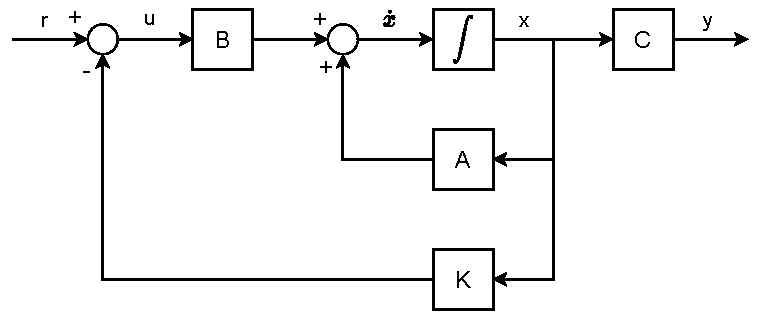
\includegraphics[width=0.65\textwidth]{Graphics/State_space_feedback.pdf}
	\caption{State space system with feedback diagram}
	\label{fig:state_space_fb}
\end{figure}






\subsection{LMI / MPC controller}
